\section{CP Model}

\subsection{Decision Variables}
The CP model relies on the following decision variables:

\begin{itemize}
    \item For each unordered pair of teams $(i,j)$ we define $\text{\textbf{period}}_{i,j} \in P$ as the slot in which team $i$ plays against team $j.$
    \item Similarly, for each unordered pair of teams $(i,j)$ we define the variables $\text{\textbf{home}}_{i,j}\in \{0, 1\}$ in such a way that $\text{home}_{i,j}=1$ when $i$ plays against $j$ at home.
\end{itemize}

Moreover, using the previously described \emph{circle method}, all week assignments are precomputed and passed to the model in the variables $\text{\textbf{week}}_{i,j} \in W$, where $\text{week}_{i,j} = w$ means that $i$ plays against $j$ in week $w$.

\subsection{Objective Function}
As already described above, the objective function is defined as
\[
\max_{t \in T} \, |H_t - A_t|,
\]
where \(H_t\) is the number of home games of team \(t\), \(A_t\) is the number of away games of team \(t\), and \(T\) is the set of teams.

In the CP model, the number of games each team plays at home and away are stored in two arrays:
\[
\forall t \in T \quad \mathtt{home\_count[t]} \in \{1, \dots, n-1\}, 
\qquad
\mathtt{away\_count[t]} \in \{1, \dots, n-1\}.
\]
The imbalance for each team is stored in
\[
\mathtt{imbalance[t]} = \lvert \mathtt{home\_count[t]} - \mathtt{away\_count[t]} \rvert
\]
and the optimization variable is taken as the $\text{max}$ over the array.

A final consideration regarding the objective function is that the CP models performed significantly better when switching from minimizing the sum of home–away imbalances to minimizing the maximum imbalance.

\subsection{Constraints}
Thanks to the previously described \emph{circle method} only two constraints had to be implemented to solve the problem in a consistent way:

\textbf{Each team plays at most twice in the same period:}
\[
\forall\, t \in T,\; \forall\, p \in P:\quad 
\sum_{j \in T \setminus \{t\}} \chi_{\{\text{period}_{t,j} = p\}} \;\leq\; 2
\]
We implemented this constraint using the global constraint \texttt{count\_geq}, which yielded better results than both the intuitive formulation and the alternative global constraint \texttt{global\_cardinality}.

\textbf{Each period in each week contains exactly one match:}
\[
\forall\, w \in W,\;
\forall\, p \in P:\quad
\sum_{\substack{(i,j) \in M}}
\chi_{\{\,\text{week}_{i,j} = w \,\wedge\, \text{period}_{i,j} = p\,\}} = 1,
\]
where $M$ is the set of all the possible matches: \[
M \;=\; \bigl\{\,(i,j) \;:\; i,j \in T,\; i<j \,\bigr\}.
\]
We tried to tackle this constraint using the global constraint \texttt{alldifferent} but it weakened the performance on basically all instances, which is why we didn't implement this constraint using the available global one.

Additional constraints were required due to the way we defined the decision variables. Specifically, we allowed the slot variable to take the value $0$, even though it does not correspond to a valid slot in which teams can play. Furthermore, the slot matrix must be symmetric, and the home team assignment also exhibits a particular structure by design:
\begin{itemize}
    \item $\forall\, t \in T:\quad \text{period}_{t,t} = 0$
    \item  $\forall\, i,j \in T,\, i \ne j:\;
\begin{aligned}
& \text{period}_{i,j} \ne 0,\\
& \text{period}_{i,j} = \text{period}_{j,i},\\
& \text{home}_{j,i} = 1 - \text{home}_{i,j}
\end{aligned}$
\end{itemize}

\subsubsection*{Symmetry Breaking Constraints}
We identified some symmetries in the problem that, if left unaddressed,  enlarged the search space explored by the solver. To reduce redundant exploration, we introduced symmetry-breaking constraints:

\textbf{SB1: Fixing the slots of the first team:}
\[
\forall\, t \in T:\quad \text{period}_{1,t} \le \text{period}_{1,t+1}
\]

This constraint ensures that the slots assigned to the first team are strictly increasing, effectively removing symmetries that arise from permuting slot orders. We implemented it using the MiniZinc global constraint $\mathtt{increasing}.$

\textbf{SB2: Team 1's home/away pattern is fixed:}
\[
\forall\, w \in W:\quad
\text{home}_{1,\, w+1} =
\begin{cases}
1, & 1 \le w \le \lfloor \tfrac{\text{num\_teams}}{2} \rfloor,\\[2mm]
0, & \lfloor \tfrac{\text{num\_teams}}{2} \rfloor + 1 \le w \le \text{num\_teams}-1
\end{cases}
\]

This constraint eliminates symmetries that come from flipping home-away status forcing the first team to play the first half of the season at home and the second away.

\textbf{SB3: Imbalance ordering:}  

\[
\forall\, t \in T:\quad \text{imbalance}_t \ge \text{imbalance}_{t+1}
\]

This last symmetry breaking constraint binds the imbalance array to be decreasing and was of course tested only on the optimization version of the problem.

\subsection{Validation}
The models were implemented in MiniZinc and coupled with a Python script that takes the input parameters, determines week assignments, and subsequently executes the corresponding MiniZinc model.

\subsubsection{Experimental design}
We experimented our models using \textbf{Gecode} and \textbf{Chuffed} with different search strategies. All experiments were conducted respecting the given timeout of $300\,\mathrm{s}$, with the solvers in their sequential version and using $42$ as \texttt{random\_seed} in order to obtain a deterministic behavior.

\subsubsection{Experimental Results (Decision version)}

In Figure~\ref{fig:solver_strategies}, we present the results for the decision version of the problem. The best configuration combines Chuffed with the random-order variable selection heuristic and Luby restarts, using a restart scale of $50$. Another clear observation is that Chuffed consistently outperforms Gecode. Overall, the results are very similar to those of the optimization version, which is why the discussion of the chosen approaches is deferred to the following section.

\begin{figure}[h!]
    \centering
    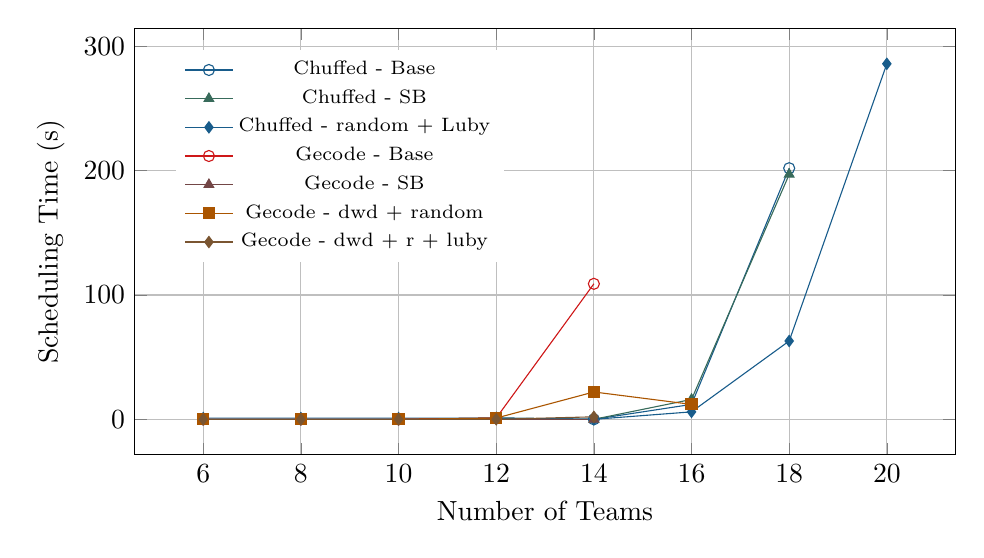
\begin{tikzpicture}
        \begin{axis}[
            xlabel={Number of Teams},
            ylabel={Scheduling Time (s)},
            grid=major,
            width=12cm,
            height=7cm,
            legend style={
                at={(0.05,0.95)},   % 5% from left, 95% from bottom
                anchor=north west,  % aligns the top-left of the legend to this             point
                font=\scriptsize,   % keeps it small
                draw=none            % optional: removes the box around legend
                },
        ]

        % Solver 1 (4 strategies) - blue shades
        \addplot[color={rgb:red,31;green,120;blue,180}, mark=o] coordinates {(6,0) (8,0) (10, 0) (12,1) (14,0) (16,12) (18,202)};
        \addlegendentry{Chuffed - Base}

        \addplot[color={rgb:red,102;green,194;blue,165}, mark=triangle*] coordinates {(6,0) (8,0) (10, 0) (12,1) (14,0) (16,16) (18,197)};
        \addlegendentry{Chuffed - SB}

        \addplot[color={rgb:red,31;green,120;blue,180}, mark=diamond*] coordinates {(6,1) (8,1) (10, 1) (12,1) (14,0) (16,6) (18,63) (20,286)};
        \addlegendentry{Chuffed - random + Luby}
        % Solver 2 (5 strategies) - red shades
        \addplot[color={rgb:red,227;green,26;blue,28}, mark=o] coordinates {(6,0) (8,0) (10, 0) (12,1) (14,109)};
        \addlegendentry{Gecode - Base}

        \addplot[color={rgb:red,251;green,154;blue,153}, mark=triangle*] coordinates {(6,0) (8,0) (10, 0) (12,0) (14,0)};
        \addlegendentry{Gecode - SB}

        \addplot[color={rgb:red,255;green,127;blue,0}, mark=square*] coordinates {(6,0) (8,0) (10, 0) (12,1) (14,22) (16,12)};
        \addlegendentry{Gecode - dwd + random}

        \addplot[color={rgb:red,255;green,178;blue,102}, mark=diamond*] coordinates {(6,0) (8,0) (10, 0) (12,0) (14,2)};
        \addlegendentry{Gecode - dwd + r + luby}

        \end{axis}
    \end{tikzpicture}
    \caption{Decision version: runtime in seconds for different solving configurations.}
    \label{fig:solver_strategies}
\end{figure}

\subsubsection{Experimental Results (Optimization version)}

Our first objective was to evaluate the impact of the proposed symmetry-breaking constraints. As shown in Table~\ref{cp-opt-results}, the inclusion of symmetry breaking yields clear benefits for both Gecode and Chuffed. In particular, Chuffed was able to solve the case $n=16$ to optimality, which was not possible without symmetry breaking and it found a better solution for $n=18$. Similarly, Gecode, when combined with symmetry breaking, successfully solved the case $n=14$ to optimality. Among the three symmetry-breaking strategies described before, the best performance was obtained using the first two, while the third did not lead to any improvement, which is why we did not use it.

Having established the advantages of symmetry breaking, we next investigated alternative search strategies to further enhance performance of both solvers. All subsequent experiments were conducted with symmetry breaking enabled.

For the optimization version with Chuffed, we were not able to identify search strategies that improved the model’s solutions, highlighting the effectiveness of Lazy Clause Generation. Among the tested configurations, the best was \texttt{random\_order} for variable selection combined with a \texttt{Luby$(50)$} restart strategy. We also experimented with \texttt{first\_fail}, but regardless of the chosen value-assignment heuristic, no improvement was observed, although \texttt{indomain\_split} performed slightly better than the others.

We additionally tested enabling free search, allowing the solver to switch between the specified search annotations and its default search. However, this significantly degraded performance: in fact, the models were unable to solve even the case $n=16$ to optimality.

For Gecode, we initially experimented with the \texttt{first\_fail} variable selection heuristic, but it did not yield any performance improvement. Switching to the domain over weighted degree heuristic, combined with random value assignment, we obtained a significant improvement. Using this approach, Gecode was able to solve instances up to $n=16$ optimally, although, the time required to solve $n=14$ increased noticeably.

We also attempted to combine this strategy with restarts, specifically \texttt{Luby}, but the results weakened. This trend was consistent across several restart scales arbitrarily chosen within $[20,150]$.

Additionally, we evaluated the large neighborhood search (LNS) strategy; however, it provided no benefit regardless of the retainment percentage. In fact the results were the same as without it. As to be expected, this approach was only tested for the optimization version of the problem.

Overall, Chuffed consistently outperformed Gecode, producing better results across nearly all non-trivial instances, with the exception of some faster solutions that Gecode was able to find for $n=16$. 

\begin{table}[h!]
\centering
\resizebox{\textwidth}{!}{%
\begin{tabular}{c|ccc|cccc}
\toprule
\multirow{2}{*}{\textbf{n}} & \multicolumn{3}{c|}{\textbf{Chuffed}} & \multicolumn{4}{c}{\textbf{Gecode}} \\
\cmidrule(lr){2-4} \cmidrule(lr){5-8}
 & Base & SB & random+luby(50) & Base & SB & dwd+random & dwd+r+luby(50) \\
\midrule
10 & $0\|\mathbf{1}$ & $0\|\mathbf{1}$ & $0\|\mathbf{1}$ & $0\|\mathbf{1}$ & $0\|\mathbf{1}$ & $0\|\mathbf{1}$ & $0\|\mathbf{1}$\\
12 & $1\|\mathbf{1}$ & $1\|\mathbf{1}$ & $2\|\mathbf{1}$ & $1\|\mathbf{1}$ & $0\|\mathbf{1}$ & $1\|\mathbf{1}$ & $1\|\mathbf{1}$\\
14 & $1\|\mathbf{1}$ & $6\|\mathbf{1}$ & $6\|\mathbf{1}$ & $300\|7$ & $0\|\mathbf{1}$ & $36\|\mathbf{1}$ & $12\|\mathbf{1}$\\
16 & $300\|3$ & $22\|\mathbf{1}$ & $87\|\mathbf{1}$ & $\text{N/A}$ & $\text{N/A}$ & $14\|\mathbf{1}$ & $300\|9$\\
18 & $300\|11$ & $300\|5$ & $300\|7$ & $\text{N/A}$ & $\text{N/A}$ & $\text{N/A}$ & $\text{N/A}$\\
\bottomrule
\end{tabular}
}
\caption{Optimization version: runtime in seconds and found objective value for different combinations of models, solvers and search strategies. Smaller instances ($6,8$) are left out because all configurations solved them instantly.}
\label{cp-opt-results}
\end{table}
